\section{ALMOS version Francois}

But: trouver une méthode pour exploiter toute la mémoire physique disponible

\begin{itemize}

  \item Francois a conservé l'adressage du noyau en mode virtuel, mais il a
    réduit son espace à 1Go.
  
  \item Il a réparti le mapping de ce giga-octet entre tous les clusters. Sur
    une archi TSAR (256 clusters, 1To de mémoire), ca donne 4Mo d'espace virtuel
    appartenant au noyau \textbf{par cluster}. \todo{On ne compte pas la place
    du réplica noyau.}

  \item la table des pages et la tables de descripteurs de pages prennent de la
    place (voire beaucoup). Pour la table des pages, c'est \textbf{8Mo
    maximum}\footnote{La table est entièrement remplie. \todo{Faudra expliquer
    pourquoi 8Mo avec le schéma de traduction d'adresse dans TSAR}}, et les
    descripteurs de pages physique, c'est \textbf{14Go} (56Mo par cluster). Cet
    espace ne peut pas être
    réduit car dans ALMOS, on a choisi de décrire \textbf{toutes les pages},
    quelles sont occupées ou non. Donc, pour décrire 1To de mémoire, on a besoin
    de 14Go.

  \item tout ca ca ne passe pas à l'échelle, puisqu'on a seulement 4Mo d'espace
    adressable  pour le noyau dans chaque cluster. Donc, Francois a passé ces
    deux structures en \textbf{adressage physique}. Comme on peut  gérer 1To
    avec des adresses physique grâce au registre d'extension d'adresse des
    processeurs MIPS\footnote{les processeurs Intel et AMD supportent également
    ce mode}, alors on peut mapper directement ces deux structures dans la
    mémoire du cluster. Schématiquement, on obtient le découpage de la
    figure~\ref{fig:decoupage}

    \begin{figure}[!h]
      \centering
      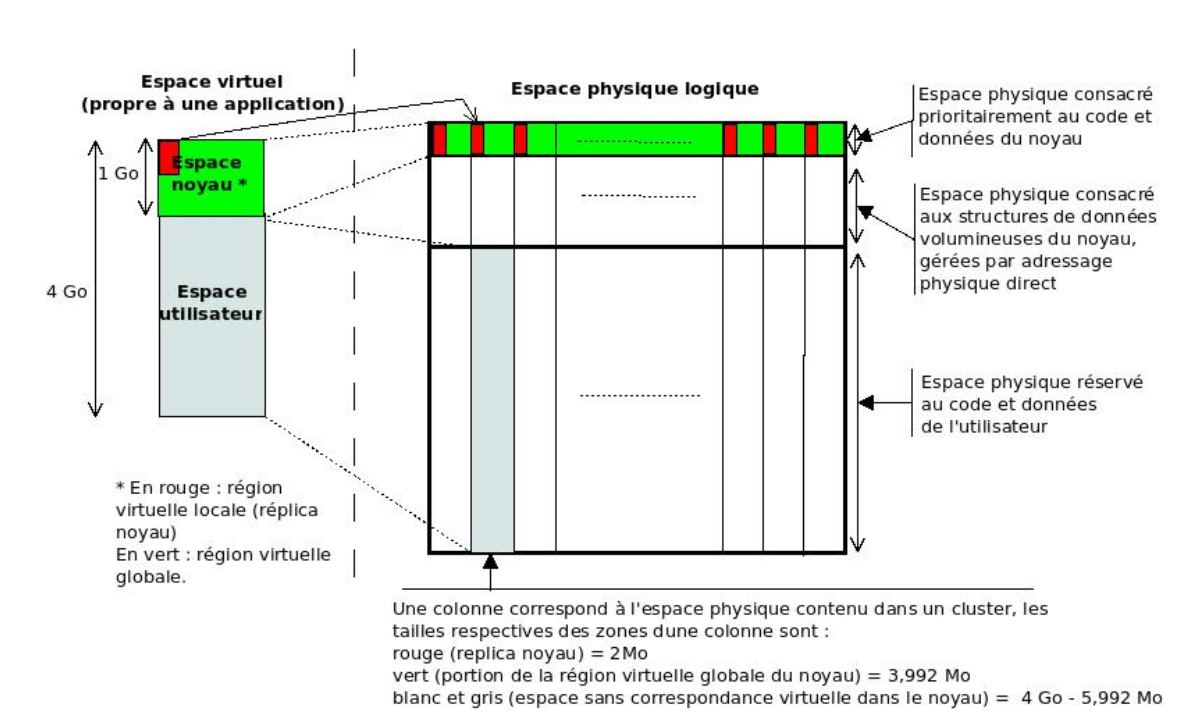
\includegraphics[scale=0.3]{decoupage}
      \label{fig:decoupage}
    \end{figure}

    En vert on a le réplica noyau, et les 4Mo d'espace virtuel, juste en dessous
    on a l'espace \textbf{non virtualisé par le noyau} mais adressable
    physiquement, et contenant les deux structures évoquées précédemment.
    Ensuite on a les 3Go de l'utilisateur.

    \textbf{Note: chaque colonne représente un cluster}

\end{itemize}

